\documentclass[12pt, a4paper, fleqn]{memoir}%makeidx

%******************************************************************************
% STYLE
%******************************************************************************
%******************************************************************************
% PACKAGES
%******************************************************************************
\usepackage{graphicx}
\usepackage{epsfig}
\usepackage{amsmath}
\usepackage{amssymb}
\usepackage{amsthm}
\usepackage{booktabs}
\usepackage{stmaryrd}
\usepackage{url}
\usepackage[figuresright]{rotating}
\usepackage{listings}
\usepackage{algorithm}
\usepackage{algpseudocode}
\usepackage{pifont}
\usepackage{ifsym}
\usepackage{relsize}
\usepackage[ansinew]{inputenc}
%\usepackage{dingbat}
\usepackage{hhline}
\usepackage{booktabs}
%\usepackage{xtab}
%\usepackage[margin=10pt,font={small,sf},labelfont=bf]{caption}
%\usepackage{tabularx}
%\usepackage{longtable}
%\usepackage{multirow}
\usepackage{color}
\usepackage{colortbl}
\usepackage{fancyvrb}
\usepackage{rotating}
\usepackage{makeidx}
\usepackage{MnSymbol}
\usepackage{textcomp}
%******************************************************************************
% INDEX GENERATION
%******************************************************************************
\makeindex

%******************************************************************************
% HYPEREF/ALGORITHM FIX
%******************************************************************************
\newcommand{\theHalgorithm}{\arabic{algorithm}}

% Konfiguration von hyperref
%\hypersetup{pdftex=true, colorlinks=true, breaklinks=true,
%   linkcolor=schwarz, menucolor=schwarz, pagecolor=schwarz, urlcolor=schwarz, citecolor=schwarz}

%******************************************************************************
% NUMBERING
%******************************************************************************
\numberwithin{algorithm}{chapter}
\numberwithin{figure}{chapter}

%******************************************************************************
% PAGE NUMBER IN BIBLIOGRAPHY
%******************************************************************************
\usepackage{citeref}
\renewcommand{\bibitempages}[1]{\newblock {\scriptsize [\mbox{cited at p.\ }#1]}}

%******************************************************************************
% PDF HYPERLINKS
%******************************************************************************
\ifpdf
  \pdfcompresslevel=9
        \usepackage[plainpages=false,pdfpagelabels,bookmarksnumbered,%
        colorlinks=true,%
        linkcolor=blue,%
        citecolor=blue,%
        filecolor=blue,%
        pagecolor=blue,%
        urlcolor=blue,%
        pdftex,
        unicode]{hyperref} 
    \input supp-mis.tex
    \input supp-pdf.tex
    \pdfimageresolution=600
    \usepackage{thumbpdf} 
\else
    \usepackage{hyperref}
\fi
\usepackage{memhfixc}

%******************************************************************************
% PAGE LAYOUT
%******************************************************************************
%\settypeblocksize{*}{32pc}{1.618}
%\setlrmargins{*}{1.47in}{*}
%\setulmargins{*}{*}{1.3}
%\setheadfoot{\onelineskip}{2\onelineskip}
%\setheaderspaces{*}{2\onelineskip}{*}
%\def\baselinestretch{1.1}
%\checkandfixthelayout



\newcolumntype{H}[1]{>{\columncolor[gray]{0.90}}p{#1}}
\newcolumntype{I}[1]{>{\centering\columncolor[gray]{0.90}}p{#1}}
\newcolumntype{q}[1]{>{\centering}p{#1}}
\renewcommand{\arraystretch}{1.25}
%******************************************************************************
% CHAPTER AND SECTION STYLE
%******************************************************************************
\makechapterstyle{mychapterstyle}{%
    \renewcommand{\chapnamefont}{\LARGE\sffamily\bfseries}%
    \renewcommand{\chapnumfont}{\LARGE\sffamily\bfseries}%
    \renewcommand{\chaptitlefont}{\Huge\sffamily\bfseries}%
    \renewcommand{\printchaptertitle}[1]{%
        \chaptitlefont\hrule height 0.5pt \vspace{1em}%
        {##1}\vspace{1em}\hrule height 0.5pt%
        }%
    \renewcommand{\printchapternum}{%
        \chapnumfont\thechapter%
        }%
}
\chapterstyle{mychapterstyle}
\setsecheadstyle{\Large\sffamily\bfseries}
\setsubsecheadstyle{\large\sffamily\bfseries}
\setsubsubsecheadstyle{\normalfont\sffamily\bfseries}
\setparaheadstyle{\normalfont\sffamily}
\makeevenhead{headings}{\thepage}{}{\small\slshape\leftmark}
\makeoddhead{headings}{\small\slshape\rightmark}{}{\thepage}

%******************************************************************************
% TABLE OF CONTENTS STYLE
%******************************************************************************
\settocdepth{subsection}
\setsecnumdepth{subsection}
\maxsecnumdepth{subsection}
\settocdepth{subsection}
\maxtocdepth{subsection}

%******************************************************************************
% COMMANDS FOR EPIGRAPHS
%******************************************************************************
\setlength{\epigraphwidth}{0.57\textwidth}
\setlength{\epigraphrule}{0pt}
\setlength{\beforeepigraphskip}{1\baselineskip}
\setlength{\afterepigraphskip}{2\baselineskip}
\newcommand{\epitext}{\sffamily\itshape}
\newcommand{\epiauthor}{\sffamily\scshape ---~}
\newcommand{\epititle}{\sffamily\itshape}
\newcommand{\epidate}{\sffamily\scshape}
\newcommand{\episkip}{\medskip}
\newcommand{\myepigraph}[4]{%
	\epigraph{\epitext #1\episkip}{\epiauthor #2\\\epititle #3 \epidate(#4)}\noindent}


%******************************************************************************
% FOOTNOTE STYLE
%******************************************************************************
\renewcommand{\thefootnote}{\fnsymbol{footnote}}

%******************************************************************************
% COLORS
%******************************************************************************
\usepackage{color}
\definecolor{greenyellow}   {cmyk}{0.15, 0   , 0.69, 0   }
\definecolor{yellow}        {cmyk}{0   , 0   , 1   , 0   }
\definecolor{goldenrod}     {cmyk}{0   , 0.10, 0.84, 0   }
\definecolor{dandelion}     {cmyk}{0   , 0.29, 0.84, 0   }
\definecolor{apricot}       {cmyk}{0   , 0.32, 0.52, 0   }
\definecolor{peach}         {cmyk}{0   , 0.50, 0.70, 0   }
\definecolor{melon}         {cmyk}{0   , 0.46, 0.50, 0   }
\definecolor{yelloworange}  {cmyk}{0   , 0.42, 1   , 0   }
\definecolor{orange}        {cmyk}{0   , 0.61, 0.87, 0   }
\definecolor{burntorange}   {cmyk}{0   , 0.51, 1   , 0   }
\definecolor{bittersweet}   {cmyk}{0   , 0.75, 1   , 0.24}
\definecolor{redorange}     {cmyk}{0   , 0.77, 0.87, 0   }
\definecolor{mahogany}      {cmyk}{0   , 0.85, 0.87, 0.35}
\definecolor{maroon}        {cmyk}{0   , 0.87, 0.68, 0.32}
\definecolor{brickred}      {cmyk}{0   , 0.89, 0.94, 0.28}
\definecolor{red}           {cmyk}{0   , 1   , 1   , 0   }
\definecolor{orangered}     {cmyk}{0   , 1   , 0.50, 0   }
\definecolor{rubinered}     {cmyk}{0   , 1   , 0.13, 0   }
\definecolor{wildstrawberry}{cmyk}{0   , 0.96, 0.39, 0   }
\definecolor{salmon}        {cmyk}{0   , 0.53, 0.38, 0   }
\definecolor{carnationpink} {cmyk}{0   , 0.63, 0   , 0   }
\definecolor{magenta}       {cmyk}{0   , 1   , 0   , 0   }
\definecolor{violetred}     {cmyk}{0   , 0.81, 0   , 0   }
\definecolor{rhodamine}     {cmyk}{0   , 0.82, 0   , 0   }
\definecolor{mulberry}      {cmyk}{0.34, 0.90, 0   , 0.02}
\definecolor{redviolet}     {cmyk}{0.07, 0.90, 0   , 0.34}
\definecolor{fuchsia}       {cmyk}{0.47, 0.91, 0   , 0.08}
\definecolor{lavender}      {cmyk}{0   , 0.48, 0   , 0   }
\definecolor{thistle}       {cmyk}{0.12, 0.59, 0   , 0   }
\definecolor{orchid}        {cmyk}{0.32, 0.64, 0   , 0   }
\definecolor{darkorchid}    {cmyk}{0.40, 0.80, 0.20, 0   }
\definecolor{purple}        {cmyk}{0.45, 0.86, 0   , 0   }
\definecolor{plum}          {cmyk}{0.50, 1   , 0   , 0   }
\definecolor{violet}        {cmyk}{0.79, 0.88, 0   , 0   }
\definecolor{royalpurple}   {cmyk}{0.75, 0.90, 0   , 0   }
\definecolor{blueviolet}    {cmyk}{0.86, 0.91, 0   , 0.04}
\definecolor{periwinkle}    {cmyk}{0.57, 0.55, 0   , 0   }
\definecolor{cadetblue}     {cmyk}{0.62, 0.57, 0.23, 0   }
\definecolor{cornflowerblue}{cmyk}{0.65, 0.13, 0   , 0   }
\definecolor{midnightblue}  {cmyk}{0.98, 0.13, 0   , 0.43}
\definecolor{navyblue}      {cmyk}{0.94, 0.54, 0   , 0   }
\definecolor{royalblue}     {cmyk}{1   , 0.50, 0   , 0   }
\definecolor{blue}          {cmyk}{1   , 1   , 0   , 0   }
\definecolor{cerulean}      {cmyk}{0.94, 0.11, 0   , 0   }
\definecolor{cyan}          {cmyk}{1   , 0   , 0   , 0   }
\definecolor{processblue}   {cmyk}{0.96, 0   , 0   , 0   }
\definecolor{skyblue}       {cmyk}{0.62, 0   , 0.12, 0   }
\definecolor{turquoise}     {cmyk}{0.85, 0   , 0.20, 0   }
\definecolor{tealblue}      {cmyk}{0.86, 0   , 0.34, 0.02}
\definecolor{aquamarine}    {cmyk}{0.82, 0   , 0.30, 0   }
\definecolor{bluegreen}     {cmyk}{0.85, 0   , 0.33, 0   }
\definecolor{emerald}       {cmyk}{1   , 0   , 0.50, 0   }
\definecolor{junglegreen}   {cmyk}{0.99, 0   , 0.52, 0   }
\definecolor{seagreen}      {cmyk}{0.69, 0   , 0.50, 0   }
\definecolor{green}         {cmyk}{1   , 0   , 1   , 0   }
\definecolor{forestgreen}   {cmyk}{0.91, 0   , 0.88, 0.12}
\definecolor{pinegreen}     {cmyk}{0.92, 0   , 0.59, 0.25}
\definecolor{limegreen}     {cmyk}{0.50, 0   , 1   , 0   }
\definecolor{yellowgreen}   {cmyk}{0.44, 0   , 0.74, 0   }
\definecolor{springgreen}   {cmyk}{0.26, 0   , 0.76, 0   }
\definecolor{olivegreen}    {cmyk}{0.64, 0   , 0.95, 0.40}
\definecolor{rawsienna}     {cmyk}{0   , 0.72, 1   , 0.45}
\definecolor{sepia}         {cmyk}{0   , 0.83, 1   , 0.70}
\definecolor{brown}         {cmyk}{0   , 0.81, 1   , 0.60}
\definecolor{tan}           {cmyk}{0.14, 0.42, 0.56, 0   }
\definecolor{gray}          {cmyk}{0   , 0   , 0   , 0.50}
\definecolor{black}         {cmyk}{0   , 0   , 0   , 1   }
\definecolor{white}         {cmyk}{0   , 0   , 0   , 0   } 
\definecolor{cell}          {cmyk}{0   , 0   , 0   , 0.25} 
\definecolor{stahlblau}		  {rgb} {0.2,0.56,0.84}
\definecolor{graurot}       {rgb} {0.62,0.15,0.15}
\definecolor{schwarz}       {rgb} {0.0,0.0,0.0}


%******************************************************************************
% BEGIN DOCUMENT
%******************************************************************************
\begin{document}

%******************************************************************************
% FRONT MATTER
%******************************************************************************
\frontmatter

%******************************************************************************
% EMPTY PAGE
%******************************************************************************
\pagestyle{empty}
This is actually the first page of the thesis and will be discarded after the print out. This is done because 
the title page has to be an even page. The memoir style package used by this template makes different indentations 
for odd and even pages which is usually done for better readability.  
\clearpage

%******************************************************************************
% TITLE PAGE
%******************************************************************************
\pagestyle{empty}
\rmfamily
\noindent
\begin{center}
University of Augsburg\\
Faculty of Applied Computer Science\\
Department of Computer Science\\
Bachelor's Program in Computer Science\\
\end{center}
\begin{figure}[h!]
\centering

\includegraphics[width=0.25\textwidth]{logo.png}
\end{figure}
\vfill\vfill
\begin{center}
\Large
Bachelor's Thesis\\
\end{center}
\vspace{2.0em}
\begin{center}
\Large
\LARGE Engagement Detection\\ \vspace{10pt} 
\Large Inferring conversational engagement from verbal and nonverbal behaviour
\end{center}
\vspace{2.0em}
\begin{center}
    \normalsize
    submitted by\\
    \large
    Amr Abdelraouf\\
    \normalsize
    on 31.7.2014
\end{center}
\vspace{2.0em}
\begin{center}
    \normalsize
    Supervisor:\\ 
    Prof. Dr. Elisabeth Andr\'{e} aus Augsburg
\end{center}
\begin{center}
    \normalsize
    Adviser:\\
    MSc. Tobias Baur
\end{center}
\begin{center}
    \normalsize
    Reviewers:\\
    Prof. Dr. Elisabeth Andr\'{e}\\
\end{center}
\cleardoublepage

%******************************************************************************
% ABSTRACT
%******************************************************************************
\chapter*{Abstract}
Interview skills are of utmost important for a person's career and personal image. Furthermore it is an essential matter to exude conversational engagement in an interview to give the impression of confidence and attentiveness. This thesis aims to track the engagement level of an interviewee in a mock interview situation. It tracks the verbal and nonverbal behaviour of the interviewee with respect to the ongoing context of the interview. The gathered engagement data can be further used to assess the interviewee's performance.

%******************************************************************************
% STATEMENT & DECLARATION
%******************************************************************************
\chapter*{Statement and Declaration of Consent}
\vfill
\subsubsection*{\LARGE Statement}
Hereby I confirm that this thesis is my own work and that I have documented all sources used.
\vfill
\begin{flushleft}
Amr Abdelraouf
\end{flushleft}  
\begin{flushright}
Augsburg, 3.7.2014 
\end{flushright}
\vfill
\vfill
\subsubsection*{\LARGE Declaration of Consent}
Herewith I agree that my thesis will be made available through the library of the Computer Science Department.
\vfill
\begin{flushleft}
Amr Abdelraouf
\end{flushleft}  
\begin{flushright}
Augsburg, 3.7.2014 
\end{flushright}
\vfill

%******************************************************************************
% TABLE OF CONTENTS
%******************************************************************************
\cleardoublepage
\rmfamily
\normalfont
\pagenumbering{roman}
\pagestyle{headings}
\tableofcontents


%******************************************************************************
% MAIN MATTER
%******************************************************************************
\mainmatter

%##########################################################
\chapter{Introduction}
\label{chap:Introduction}

\section{Motivation}
\label{sec:Motivation}
This thesis was proposed to help measure the engagement of an interviewee in a job interview situation. Through a simple mock interview the performance of the interviewee will be assessed. One of the most important attributes of that performance is whether or not the interviwee is engaged with and attentive to the interviewer. A simple playback of the interview coupled with the measurement of the engagement level will easily highlight the ups and downs of his/her demonstration in the mock interview.

\section{Objectives}
\label{sec:Objectives}
This thesis aims to measure the engagement levels of an interviewee through verbal and non verbal behaviour of said interview. It studies the conversational interaction with the interviewer, the responses to certain commands and behaviour during certain segments of the interview.

\section{Outline}
\label{sec:Outline}
This thesis will first discuss the theoretical background and the information gathered on this subject. It will go into the details of the work previously done. Next it will describe the setup of it's mock interview from both the interviewer and the interviewee's perspectives.

In the following section details of constitution and software workings of this thesis will be covered. First it will describe the general structure of the pipeline. Then it will describe how the inputs are processed from a bottom up approach; starting with raw sensor data and working up level by level to demonstrate how the engagement is calculated.

%##########################################################
\chapter{Theoretical Background}
\label{chap:TheoreticalBackground}

\section{Previous Work}
\label{sec:PreviousWork}

\subsection{Recognizing Engagement in Human Robot Interaction}
In \cite{rich} Rich et al. studied the engagement behaviour in a conversation between a human and a humanoid robot. Their target was to build a robot architecture that would allow the robot to mimic the conversational behaviour of a human. The attributes of the measured engagement were divided into 4 main parts:

\begin{description}
  \item[Mutual Facial Gaze] Ability of both parties to maintain eye contact.
  \item[Directed Gaze] Ability of one party to follow the gaze of the other when the other party points or gazes at a certain object in the environment.
  \item[Adjacency Pair] The ability of one party to reply sensibly to the other party's speech.
  \item[Backchanneling] During the speech of one party, the other communicates a small gesture to indicate attentiveness.
\end{description}

You will find that this thesis is heavily influenced by Rich et al.'s work, with a slight modification to the definition of the four main modules.

\subsection{Engagement Rules for Human-Robot Collaborative Interactions}
Like the previously mentioned paper, Sidner et al. \cite{sidner} worked on a robot that is to mimic human social behaviour.

The paper builds the human-robot interaction on three main pillars. Namely initiating, maintaining and terminating engagement behaviour during a conversation, understanding the speech utterance and replying accordingly, and finally the ability to take a decision and point the conversation into a certain direction.

The paper uses a set of rules to allow the robot to understand both how to engage and how to recognize engagement. The robot uses facial gaze and greeting utterances to indicate the start of a conversation. It maintains its gaze with the human conversation participant as long as the participant is speaking. To detect that the human participant wishes to disengage from the conversation the robot monitors the interlocuter's gaze; if it is set away from the robot then the desire to disengage is detected. And lastly when the robot runs out of things to say and wishes to disengage itself, it closes the conversation using a set of rules for conversation closing.

%%##########################################################
\chapter{Setup}
\label{chap:Section}

\section{Subject}
\label{sec:Subject}
The subject of our experiment is the interviewee in our mock interview. As shown in figure \ref{fig:setup_img} the subject is seated approximately 70 cm from a screen. A number of sensors are then set up to capture the needed inputs. Namely a Microsoft Kinect, an SMI Eyetracker and a microphone.

\section{Agent}
\label{sec:Agent}
There are two main softwares used to simulate the virtual interview environment. First there is Charamel. Charamel is responsible for creating the interviewers (or agents) and their surrounding environment. The scene used for this thesis consists of two virtual characters, namely Curtis and Gloria. They stand behind a desk to mimic an office interview. On the left lies a white board that is used as an object in our environment. The setting is demonstrated in figure \ref{fig:agents_img}.

The second software used is Scenemaker. Scenemaker is responsible for sending the agents actions to perform. The program consists of a state machine, each state containing a command to be executed by the agents accordingly. These commands include ordering the agents to utter a certain sentence, stop and wait for the subject to reply, perform a certain hand gesture, and so on and so forth. Scenmaker also contains a script that defines dialogues to be acted out by the agents. The agents follow the dialogue when it is referenced in one of the state machines.

\begin{figure}[h!]
    \centering
    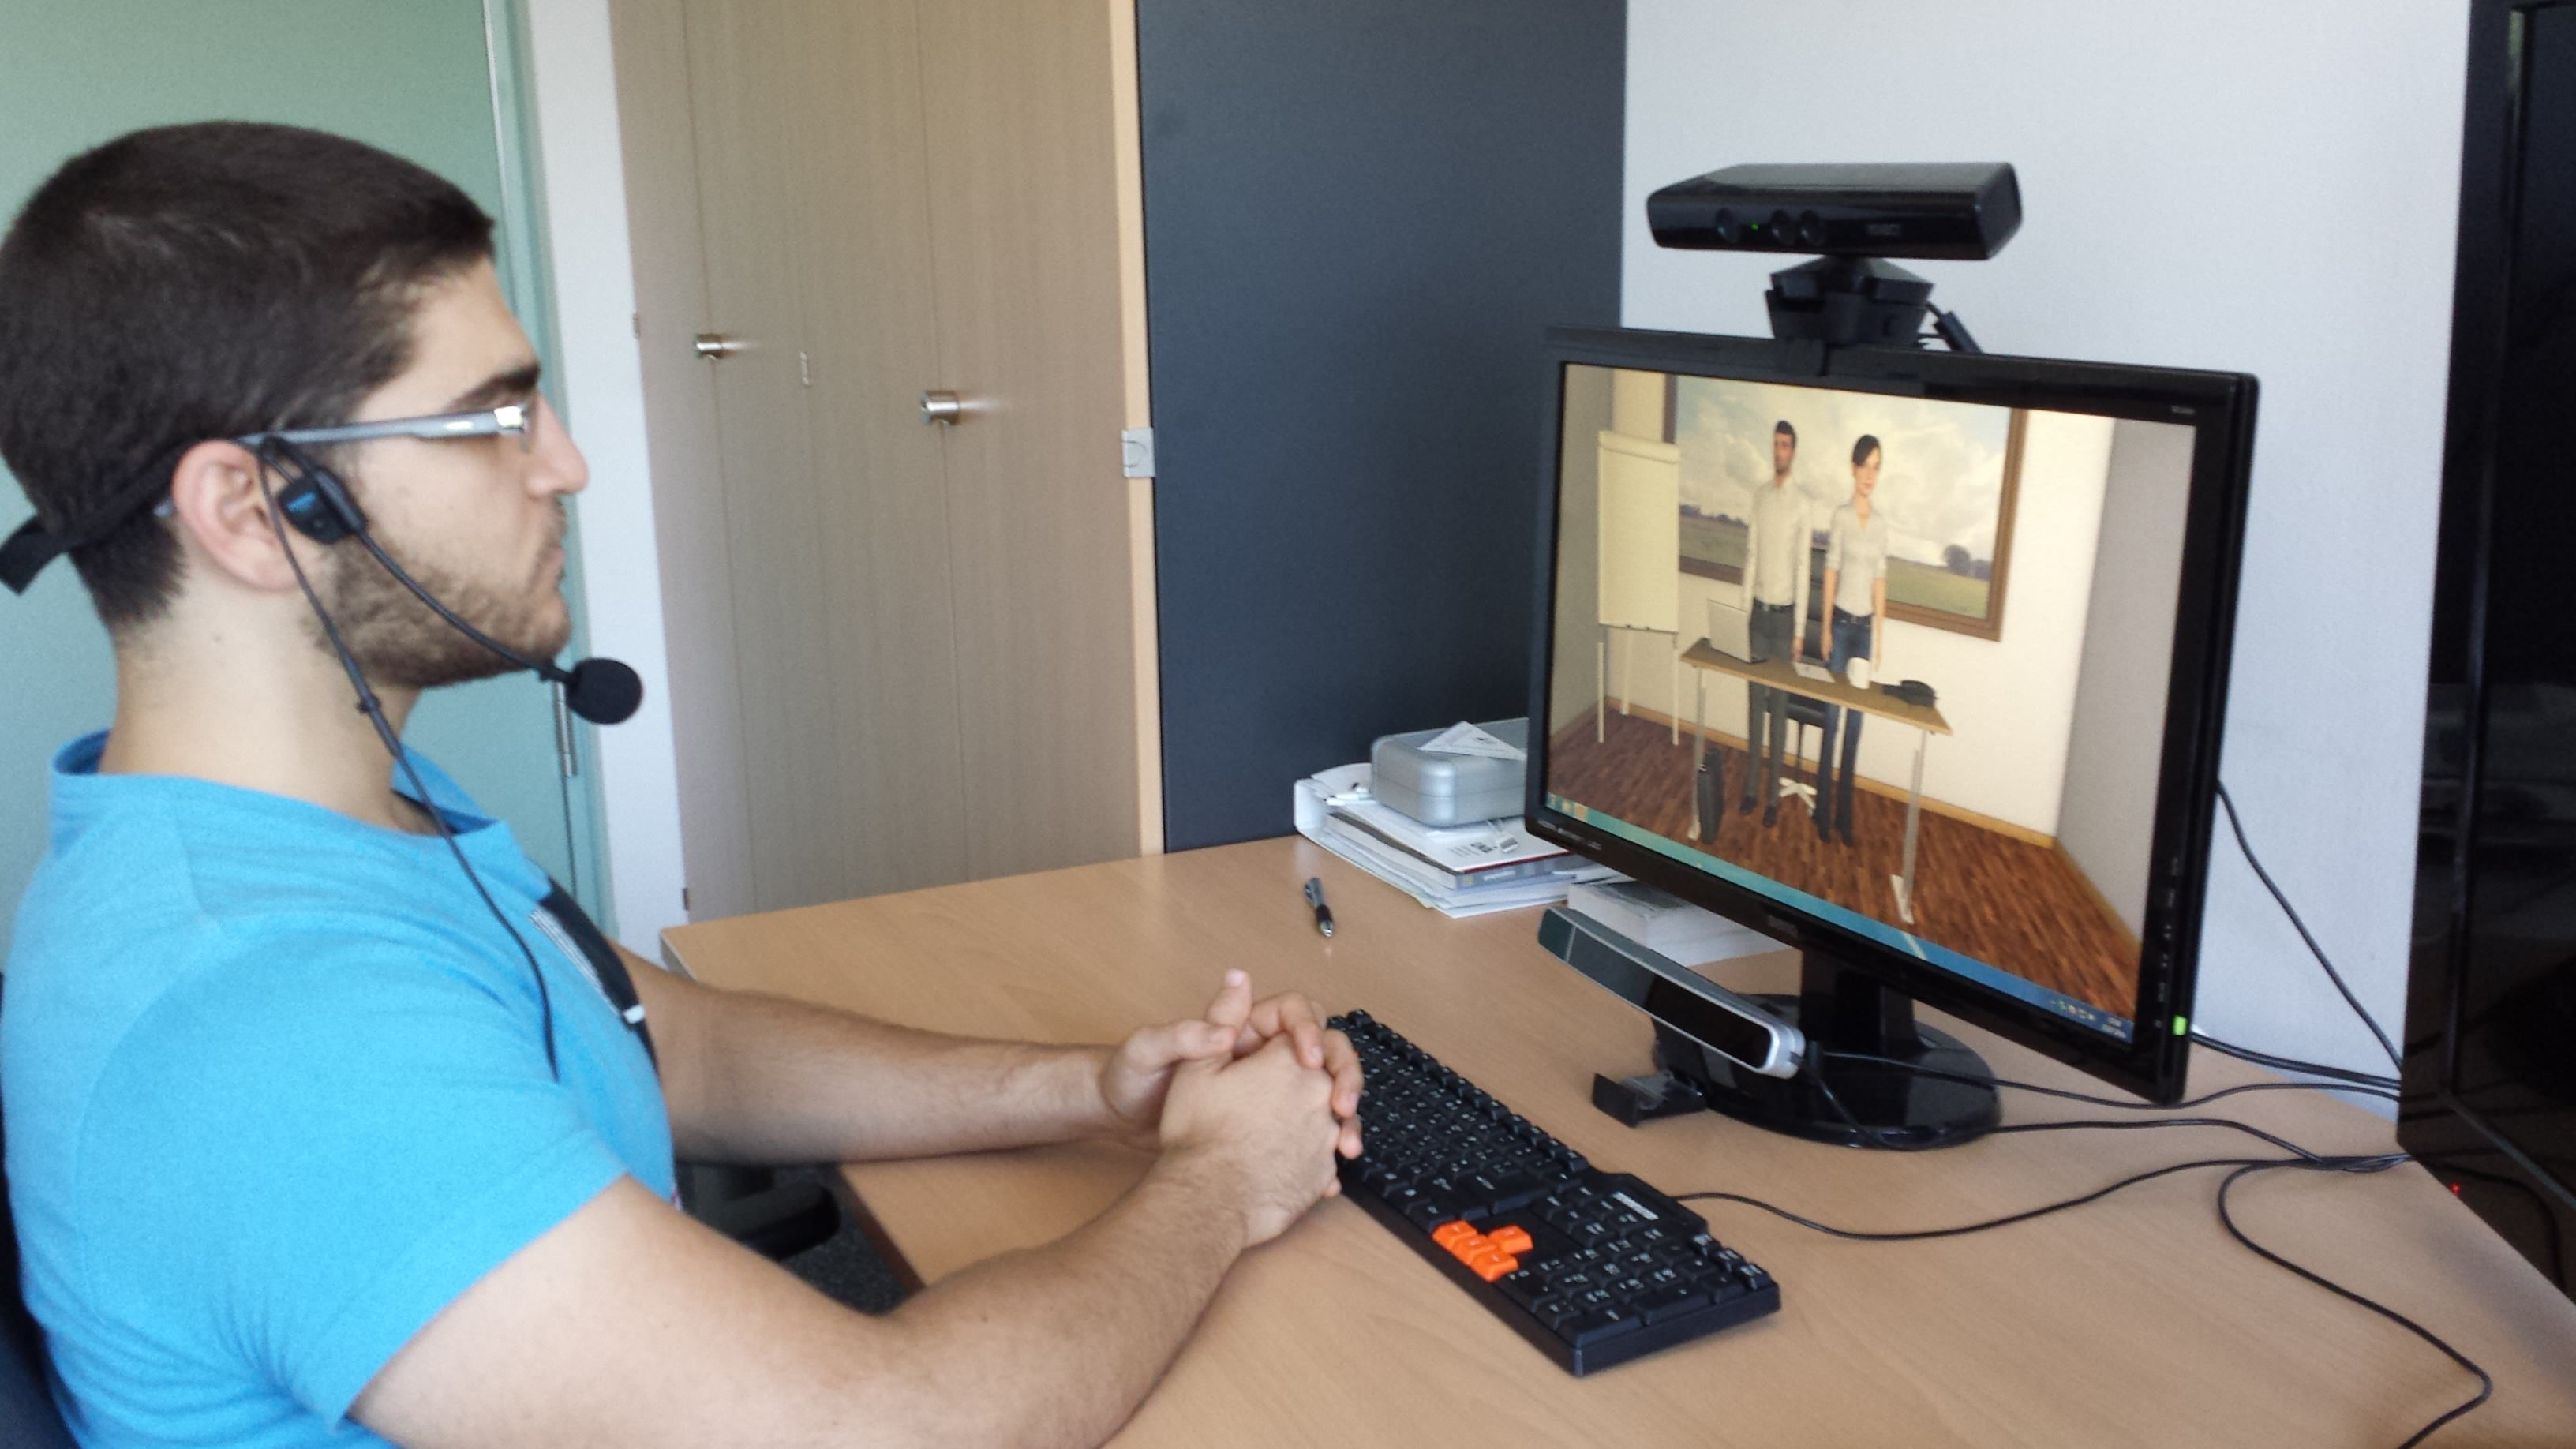
\includegraphics[width=1\textwidth]{setup}
    \caption{Interview setup}
    \label{fig:setup_img}
\end{figure}

\begin{figure}[h!]
    \centering
    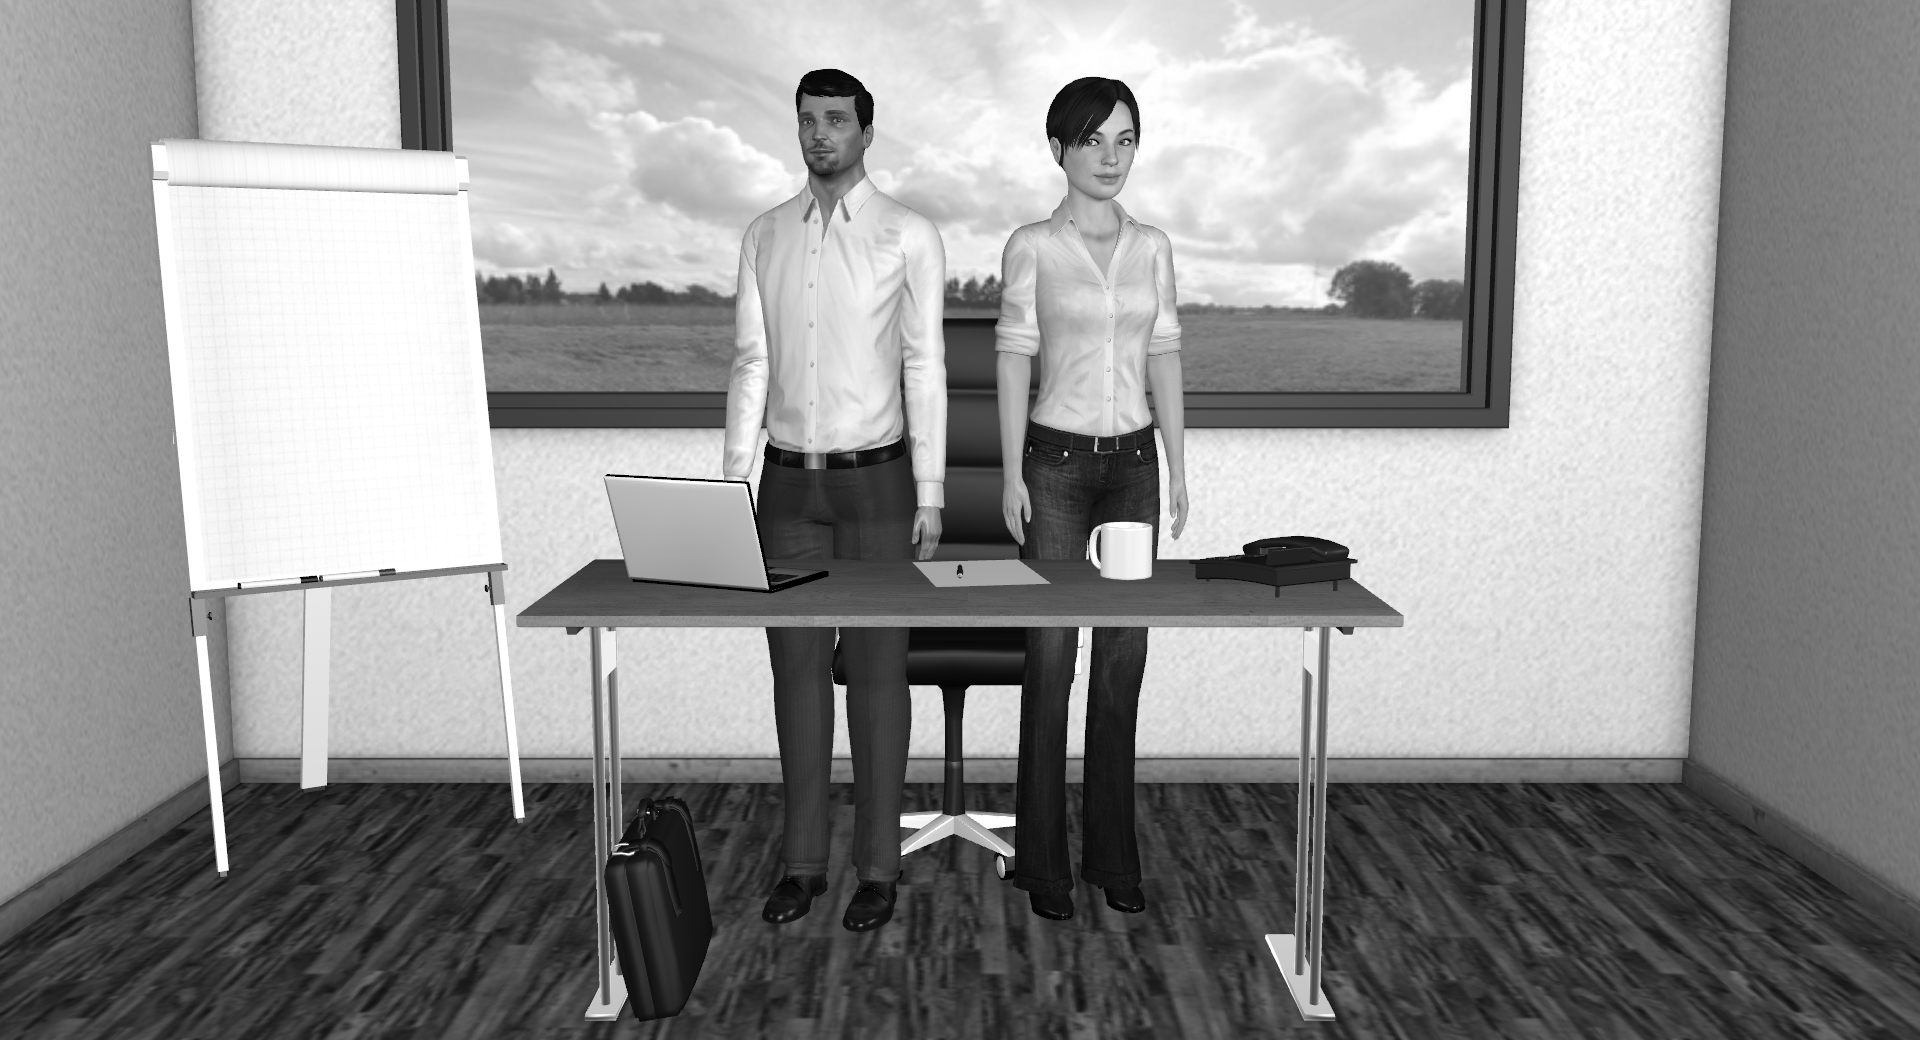
\includegraphics[width=1\textwidth]{agents}
    \caption{Virtual environment}
    \label{fig:agents_img}
\end{figure}

%%##########################################################
\chapter{Events}
\label{chap:Events}
Events are the backbone of the software workings of this thesis. Raw sensor data are converted to events that can be further processed in the software's pipeline. Furthermore external software send events to our own software over a network. These events can be displayed by themselves as output or can be used as inputs to trigger other events.

\section{Event Structure}
Events are constructs of several attributes:

\begin{description}
  \item[Time] The clock signature of when the event was triggered.
  \item[Duration] The time duration of the event.
  \item[Ptr] (Pointer) Meta data about the event.
  \item[Type] Indicates the nature of the meta data wrapped by the event.
  \item[State] A boolean flag to indicate whether the event is starting or ending.
\end{description}

In the software's pipeline events are measuerd every time cycle. A cycle of 500 ms is used.

\section{Sensors}
\label{sec:Sensors}

\subsection{Microsoft Kinect}
Kinect is a device made by Microsoft to sense 3D movements. It uses a number of cameras to detect a 3D environment; A normal VGA camera and an infrared camera that is used to measure and create a depth map.

Kinect can also track the skeletal movements of a person standing in its range. It measures the joint orientation and sends the data to the api. Kinect detects the skeletal movements of a user in two main stages. First it uses the infrared camera to create a depth map. Secondly the machine learning is used to decide whether or not the image in the depth map represents a skeleton.

In our software we are mostly interested in the movement of the subject's head. Kinect is used to detect the perpetual displacement of the subject's head which indicates that s/he is nodding. This triggers an event called \textit{HeadNod}. HeadNod is an event measured and outputed every 500 ms and its pointer contains a value from 0 to 1 which represents the probability that the subject is nodding.

\subsection{SMI Eyetracker}
The SMI Eyetracker is a plug-and-play hardware that is used to pinpoint where the user is looking. It is placed below th screen approximately 65-70 cm away from the user. After calibrating the user position with an eye tracking test a stream of x and y coordinates is sent via the SMI API to our software's pipeline. Since the machine used in this thesis runs an 64 bit operating system (which is incompatible with the SMI software), we connect the eye tracker to a separate machine. We then receive the stream via the LAN network.

Since we are dealing with a virtual agent on a screen we consider the top left corner of the screen as the (0,0) coordinate. Displacement of the subject's gaze point to the right alters the x coordinate and to the bottom affects the y coordinate.

The software defines two main rectangular areas on the screen. First is the area of the Agent's face. Second is the area of the board that is present in the environment.

When the subject's gaze point falls on the area defined for the agent's face it triggers an event called \textit{SubjectFacialGaze}. SubjectFacialGaze's pointer contains a value of either 0 or 1 indicating whether or not the subject is looking at the agent's face. When the gaze enters the facial area SubjectFacialGaze is triggered with the value 1 indicating that it has started and when the gaze leaves the facial area it is triggered with the value 0 indicating that it is complete.

If the subject's gaze falls in the area of the board the event \textit{SubjectObjectGaze} is triggered. Similar to SubjectFacialGaze, the event carries a value of either 0 or 1 indicating whether or not the subject is looking at the board. The event is prompted with pointer value 1 when the subject starts looking at the object, and triggered again with 0 when the subject directs his/her gaze away.

\subsection{Microphone}
A microphone is used to record the verbal utterances produced by the subject. When the microphone detects a voice the event \textit{vad} (which is short for Voice Activity Duration) is fired. When the voice is first detected the event's pointer carries a value of 1. When the voice activity ends the same event is triggered but with value 0 to indicate that the event is complete.

In our experiment we used a microphone mounted on a head gear to eliminate noise produced by the agents' speech utterances.

\section{Scenemaker}
\label{sec:Scenemaker}
As mentioned before in subsection \ref{sec:Agent} Scenemaker is the software used to send commands to the virtual agents. Scenemaker is also responsible for sending the events that are triggered to represent the agents' behaviour to our software's pipeline. The events can be subcategorized into two main parts: Gaze and speech.

\subsection{Gaze}
Firstly we are concerned with where the agent is looking. When the script commands the agent to looks at the subject in front of the screen the event \textit{AgentFacialGaze} is triggered. Similar to the subject's gaze events the event pointer holds the value 1 when the agent starts looking at the subject and holds the value 0 when the agent looks away from the subject's face.

Furthermore when the agent is commanded to look at the board, the event \textit{AgentObjectGaze} is triggered with a pointer value 1 or 0 indicating that the agent has started or stopped looking at the board.

\subsection{Speech}
As mentioned in \ref{sec:Agent} it was mentioned that Scenemaker contains a script. A script contains a number of dialogues and each dialogue is split into a number of sentences. When the agent starts reading a sentence the event \textit{AgentSpeech} is triggered with a pointer value of 1. When the agent finishes reading that sentence AgentSpeech is triggered with a pointer value of 0.

%%##########################################################
\chapter{Main Modules}
\label{chap:MainModules}
So to review our events, we have:

\begin{itemize}
  \item HeadNod
  \item SubjectFacialGaze
  \item SubjectObjectGaze
  \item vad
  \item AgentFacialGaze
  \item AgentObjectGaze
  \item AgentSpeech
\end{itemize}

Those events will be used as inputs for our four main modules.

\section{Mutual Facial Gaze}
\label{sec:MutualFacialGaze}
Mutual Facial Gaze is defined as the eye contact between the subject and the agent. It is necessary for the subject to direct his/her gaze at the agent's face when being addressed. The event \textit{MutualFacialGaze} is triggered with a pointer value 1 (indicating that it started) when both SubjectFacialGaze and AgentFacialGaze are ongoing. When either of the two input events are triggered with the value 0 (event ends) the event MutualFacialGaze is also ends and therefore is triggered with pointer value 0.

\begin{figure}[h!]
    \centering
    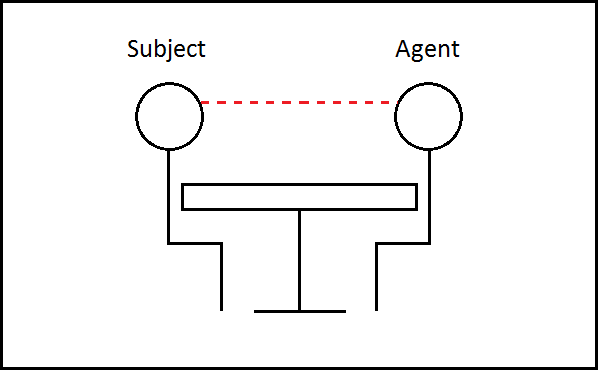
\includegraphics[width=0.6\textwidth]{MFG}
    \caption{Mutual Facial Gaze}
    \label{fig:MFG_img}
\end{figure}

\section{Directed Gaze}
\label{sec:DirectedGaze}
Directed Gaze occurs when the agent points or looks at a certain object and then the subject follows as shown in figure \ref{fig:DG_img}. In our environment the white board acts as the object. The event \textit{DirectedGaze} is triggered with pointer value 1 when both SubjectObjectGaze and AgentObjectGaze are ongoing. And triggered again with pointer value 0 when one of the two input events ends.

\begin{figure}[h!]
    \centering
    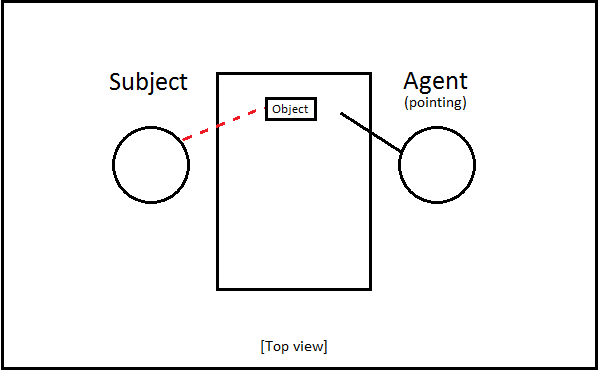
\includegraphics[width=0.6\textwidth]{DG}
    \caption{Agent points to object while subject is looking at it}
    \label{fig:DG_img}
\end{figure}

\section{Backchanneling}
\label{sec:Backchanneling}
Backchanneling is the small responses given by the subject during the time where the agent is speaking. These responses indicate that the subject is following what the agent is saying.

Here we introduce the concept of a \textit{Backchanneling Pulse}. Since backchanneling has a very short duration that usually lasts only one event cycle which is not enough time to influence the bayesian network. So instead when a backchanneling event is provoked it is outputed on 5 consecutive event cycles with pointer value 1, 0.75, 0.5, 0.25 and 0 respectively, as shown in figure \ref{fig:bcp_img}.

\begin{figure}[h!]
    \centering
    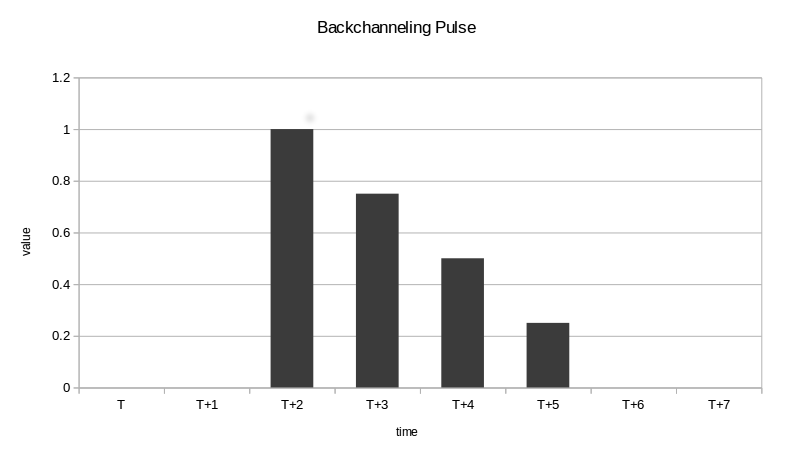
\includegraphics[width=1\textwidth]{bcp}
    \caption{Backchanneling event triggered at T+2}
    \label{fig:bcp_img}
\end{figure}

A BCPulse can be triggered by two different ways. It can be prompted when a HeadNod is detected during AgentSpeech. Or it can be set off when a vad event with a duration less than 2 seconds is detected during an AgentSpeech.

\section{Adjacency Pair}
\label{sec:AdjacencyPair}
Adjacency Pairs are defined as a speech utterance which is provoked by a previous speech utterance. For instance the answer to a question is an adjacency pair. This thesis did not go into the the semantics of natural language processing. The inputs where when the agent started and stopped speaking, and when the subject started and stopped speaking. Naturally we redefined the meaning of adjacency pairs to match our inputs.

This thesis defines adjacency pairs as one of two conversational situations:

\begin{itemize}
  \item If the subject starts speaking within a two second time window after the agent has finished its sentence it is considered an adjacency pair and a \textit{AdjacencyPair} start event is initiated. This is demonstrated in the second line in figure \ref{fig:AdjPair_img}.
  \item An AdjacencyPair start event is triggered the subject starts speaking right before the agent finished speaking as depicted in the second line of figure \ref{fig:AdjPair_img}. This is to mostly account for the delay in the pipeline between the triggering of the AgentSpeech end event and the vad start event.
\end{itemize}

AdjacencyPair end events are triggered when the vad event associated with the AdjacencyPair event ends.

\begin{figure}[h!]
    \centering
    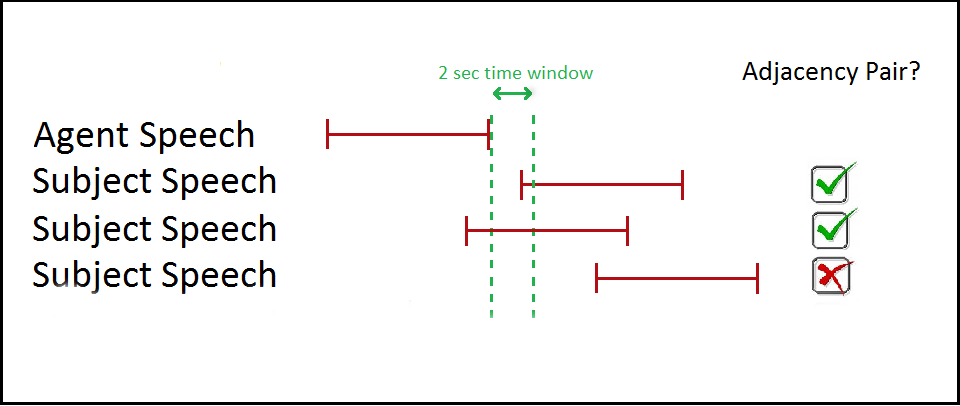
\includegraphics[width=1\textwidth]{AP}
    \caption{Adjacency Pair}
    \label{fig:AdjPair_img}
\end{figure}

%%##########################################################
\chapter{Bayesian Network}
\label{chap:BayesianNetwork}
The final stage in our pipeline is to input our four main modules as factors to calculate the engagement. This is done using a bayesian network. The bayesian network was out of this thesis work's scope. Yet it is essential for this thesis to mention and explain how the bayesian network operates as it is the bridge between the work done in this thesis and the calculation of the final engagement value.

A Bayesian network is a statistical model that is represented using a directed graph. Each node in the graph represents a variable. Each directed edge from node A to node B represents a relation between the two variables. It denotes that the value of A directly affects the value of B. Moreover when an a change occures to node B (a change independent of node A) the bayesian networks adjusts the value of node A according to the relationship defined between A and B. So a directed edge indicates both a direct and indirect relation between two nodes.

Each node has an associated probability table. Each entry in the table contains the probability of the value of its associated node given the values of its input nodes. If node B has no other directed edges pointing to it then it would have 2 entries in its probability table indicating the value of B when A is present and when A is unpresent.

Figure \ref{fig:BN_start_state_img} shows the start state of the bayesian network used in our software. The starting values of the probability are set intuitively but non of them are used since all of the leaves in this bayesian network's tree are connected to external softwares which provide the real time values. This thesis is mainly concerned with the relationship between the nodes of the four main states (nodes MutualFacialGaze, DirectedGaze, Backchanneling, and AdjacencyPair) and the Engagement node.

\begin{figure}[h!]
    \centering
    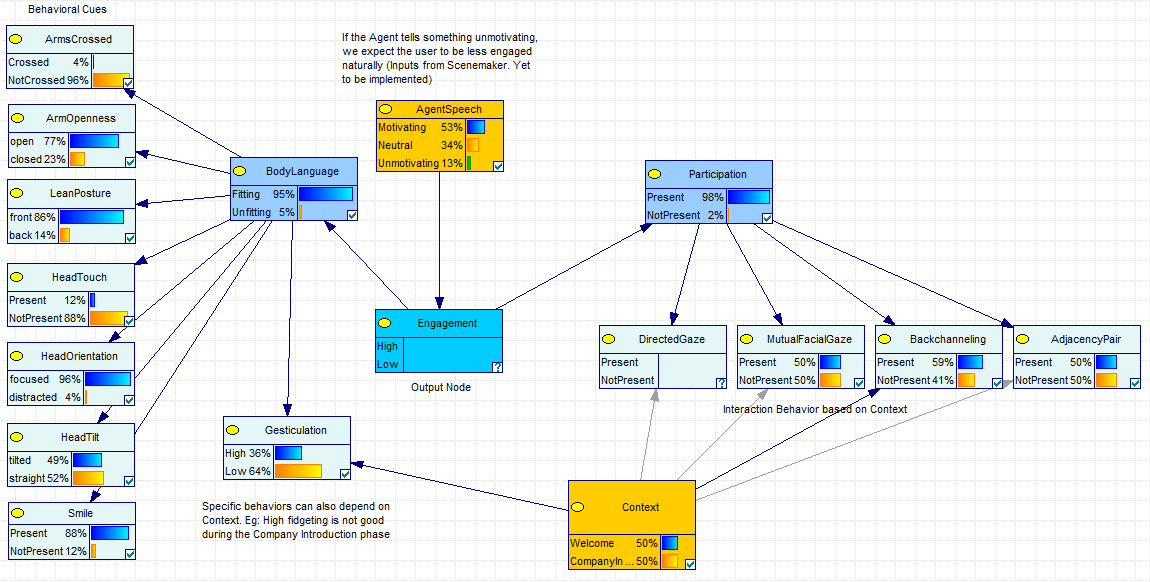
\includegraphics[width=1\textwidth]{BN_start_state}
    \caption{Bayesian network start state}
    \label{fig:BN_start_state_img}
\end{figure}

As mentioned before each node has an associated probability table. Figure \ref{fig:BN_probability_table} shows the probability table of node Backchanneling. The node has two input directed edges coming from the nodes Participation and Context. The set probability of Backchanneling when participation is present and the context is welcome is 0.51. The probability of Backchanneling when participation is not present and context is companyintro (company introduction phase) is 0.01, and so on and so forth.

\begin{figure}[h!]
    \centering
    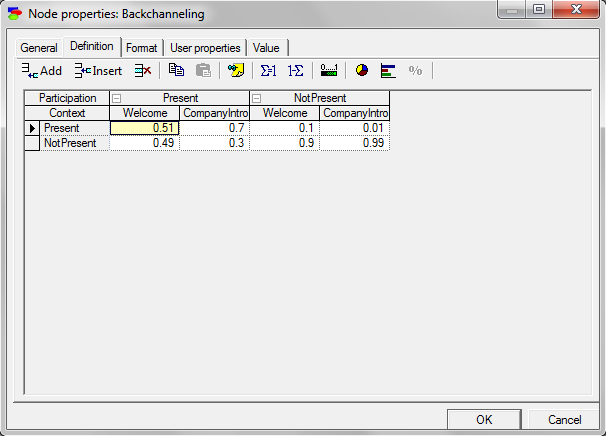
\includegraphics[width=1\textwidth]{BN_probability_table}
    \caption{Probability table of Backchanneling node}
    \label{fig:BN_probability_table}
\end{figure}

To set the values for the nodes our software communicates the output events to the bayesian network. As mentioned before each event carries an associated value from 0 to 1. These values are used to set evidence for the values in the nodes. For example if a mutual facial gaze occurs a MutualFacialGaze event is prompted with a pointer value of 1. The bayesian network then sets the evidence for the node MutualFacialGaze as Present = 100\%, notPresent = 0\%.

Figure \ref{fig:BN_state} depicts an example of the state of the bayesian network at a given intsance. It mimics a hypothetical situation during the interview from the point of view of the nodes of the four main modules only. All the other nodes are left untouched and contain their default values. In this case the MutualFacialGaze and AdjacencyPair is present (and therefore set at 100\%) while the DirectedGaze and Backchanneling (both set at 0\%) are not. This indicates a situation where the subject is facing the Agent and for example answering its question. By only setting these two variables the bayesian network back propagated through the Participation node to the Engagement node, calculating an engagement probability of 78\%. This is of course very intuitive since a subject facing and replying to an agent is clearly engaged in conversation.

\begin{figure}[h!]
    \centering
    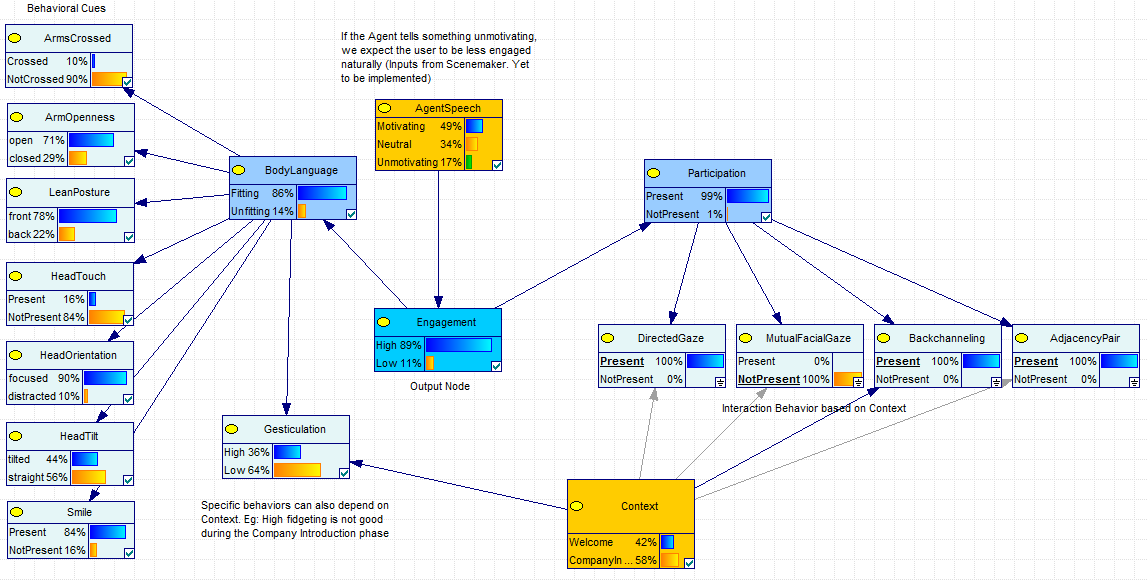
\includegraphics[width=1\textwidth]{BN_state}
    \caption{Instance of bayesian network}
    \label{fig:BN_state}
\end{figure}


%%##########################################################
\chapter{Summary}
\label{Summary}
To reach the thesis's aim of detecting the engagement of an interviewee in an interview situation we have devised a setup which consists of a hardware and software component.

The hardware component refers to the setup of the experiment. The interviewee is seated across two virtual agents present on a screen. Attached to the top of the screen a Microsoft Kinekt which mainly aims to track the movement of the subject's head. On the bottom of the screen lies an SMI Eyetracker used to track the subject's gaze and feed gaze point co-ordinates to our software. And finally a microphone that is used to record the subject's speech utterances.

\begin{figure}[h!]
    \centering
    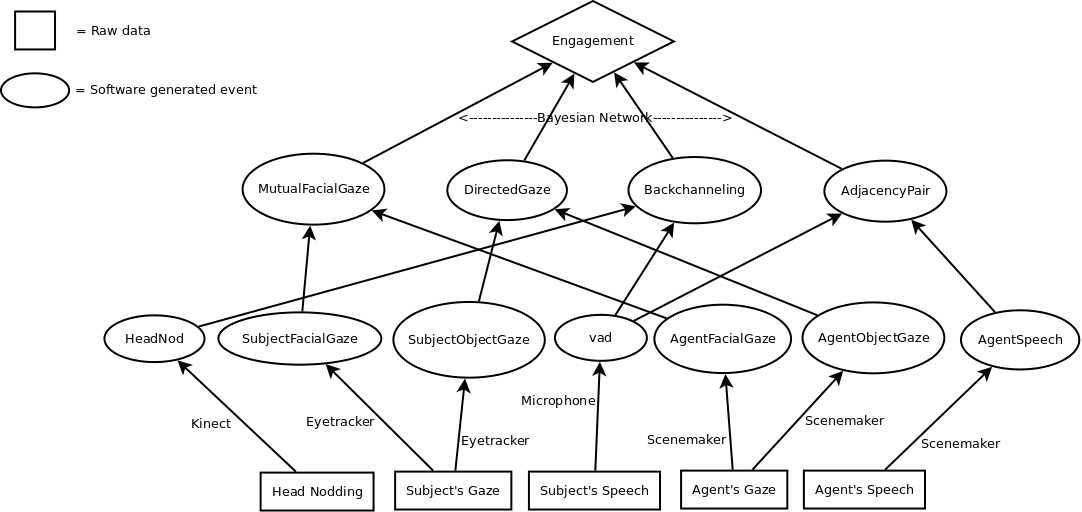
\includegraphics[width=1\textwidth]{Summery_diagram}
    \caption{Software pipeline}
    \label{fig:Summery_diagram}
\end{figure}

The pipeline of our software is topological. As shown in figure \ref{fig:Summery_diagram} the software's pipeline starts with the raw input data given by both the subject and the agent. Namely the subject's head nod, gaze, and speech which are captured by the Microsoft Kinekt, the SMI Eyetracker and the microphone respectively, and the agent's gaze and speech, which are both data that is generated by the external software Scenemaker.

The next level of the pipeline includes the basic events. \textit{HeadNod} which is controlled by the subject's nodding, \textit{SubjectFacialGaze} and \textit{SubjectObjectGaze}, triggered by the location of the subject's gaze. \textit{vad} (Voice Activity Duration) that is prompted when the subject speaks. As for the agent there are \textit{AgentFacialGaze}, \textit{AgentObjectGaze}, and \textit{AgentSpeech} which are activated by where the agent's looking and whether or not it is speaking.

Next comes the four main modules in this thesis. Those are the four main phenomena that the software tries to capture. First there is \textit{MutualFacialGaze}, which can be thought of as the eye contact between the subject and the agent. This is controlled by the basic events SubjectFacialGaze and AgentFacialGaze. Next there is \textit{DirectedGaze}. It is triggered when the subject follows the gaze of the agent when it directs him to a certain object. This event is controlled by SubjectObjectGaze and AgentObjectGaze. Then comes \textit{Backchanneling}. Backchanneling is an event in which the subject directs a brief verbal event or gestural communication back to the agent during the agent's speech. This event indicates that the subject is following what the agent is saying. Backchanneling is controlled by HeadNod, vad, and AgentSpeech. Finally comes \textit{AdjacencyPair} which is a speech communicated by the subject following a speech uttered by the agent. AdjacencyPair is controlled by vad and AgentSpeech.

Last level in our topology is the Engagement level. Contrary to figure \ref{fig:Summery_diagram} the four main modules are not the only contributors to the calculation of the engagement level. They are merely so from the point of view of this thesis. The main modules are inputed into the bayesian network and together with other factors calculate the level of engagement.

%******************************************************************************
% BIBLIOGRAPHY
%******************************************************************************
\bibliography{master}
\bibliographystyle{plain}

%******************************************************************************
% APPENDIX
%******************************************************************************
%\appendix
%\appendixpage*
%\chapter{First Appendix}

%******************************************************************************
% BACK MATTER
%******************************************************************************
\backmatter

%******************************************************************************
% LIST OF SYMBOLS
%******************************************************************************
%\normalfont
%\clearpage
%\chapter[List of Symbols and Abbreviations]{List of Symbols and Abbreviations}
%\begin{center}
%\small
%\begin{longtable}{lp{3.0in}c}
%\toprule
%\multicolumn{1}{c}{Abbreviation} & \multicolumn{1}{c}{Description}\\ \midrule\addlinespace[2pt] \endhead
%\bottomrule\endfoot
%XML & E\textbf{X}tensible \textbf{M}arkup \textbf{L}anguage \\
%XSD & \textbf{X}ML-\textbf{S}chema-\textbf{D}efinition \\
%SFXML & \textbf{S}cene\textbf{F}low E\textbf{X}tensible \textbf{M}arkup \textbf{L}anguage \\
%SFTXL & \textbf{S}cene\textbf{F}low \textbf{T}extual E\textbf{X}pression \textbf{L}anguage \\
%SCXML & \textbf{S}tate\textbf{C}hart E\textbf{X}tensible \textbf{M}arkup \textbf{L}anguage \\
%DOM & \textbf{D}ocument \textbf{O}bject \textbf{M}odel \\
%LR & \textbf{L}eft to \textbf{R}ightmost derivation \\
%LALR & \textbf{L}ook\textbf{A}head LR\\
%NPC & \textbf{N}on-\textbf{P}erson-\textbf{C}haracter\\
%ABL & \textbf{A} \textbf{B}ehavior \textbf{L}anguage\\
%\end{longtable}
%\end{center}

%******************************************************************************
% LIST OF FIGURES
%******************************************************************************
\normalfont
\clearpage
\listoffigures

%******************************************************************************
% END DOCUMENT
%******************************************************************************
\end{document}
